%!TEX root=../oi-magistr-si.tex
\setcounter{section}{18}
\section[WA2 - Cloud]{Cloud architektury, virtualizace, různá pojetí cloudových řešení, omezení cloudových aplikací, náklady na provoz, vlastnosti aplikací vhodných pro nasazení v cloud architektuře.}

% https://docs.google.com/document/d/1v3kWgsxv67yEE10eLNGlU0HIaYy_OC1C5j8QX9k9ZSg/edit?hl=en_US#

Cloud-Computing architektury můžeme rozdělit do 3 hlavních vrstev:

\begin{figure}[h!]
\centering
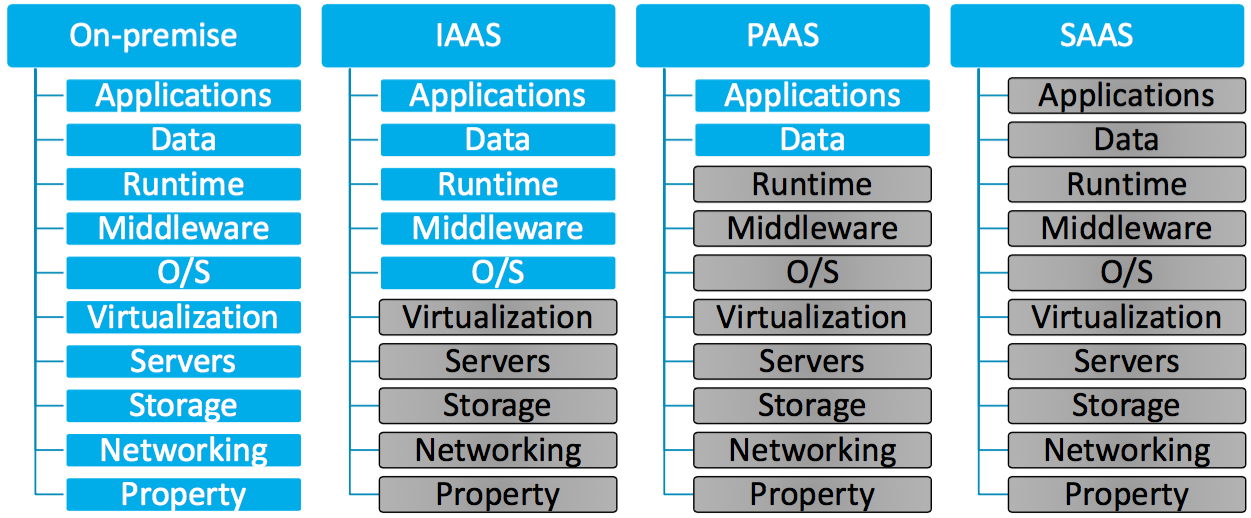
\includegraphics[width=140mm]{19/images/cloud-types}
\end{figure}


\subsection{Infrastructure as a Service (IaaS)}
Je to vlastně outsourcing výpočetního vybavení (servery, HW, síťové komponenty, storage). Poskytovatel služby je odpovědný za housing, běh a správu těchto komponent. Klient obvykle platí v modelu \textit{pay-as-you-go} či smluvním paušálem (předplatným), popřípadě kombinací obojího.
\paragraph{Příklady služeb IaaS:} Amazon EC2, Amazon S3, GTS Managed Server - Virtual Server.

\subsection{Platform as a Service (PaaS)}
Provider poskytuje přístup ke computing platformě či computing stacku (množina softwarových subsystemů, které poskládáte do výsledné služby). Jako v případě IaaS máte k dispozici servery, storage, ale omezené vybranou platformou. Zatímco na IaaS můžete v rámci virtuálního prostředí provozovat téměř jakoukoliv aplikaci, volba platformy (operacniho systemu ci programovaciho jazyka) je plně v kompetenci klienta, u PaaS jste již vázáni kompletní platformou.

\paragraph{Nebezpečí Vendor Lock-In} jste omezeni platformou poskytovate (.NET na MS Azzure), proprietární službou či množinou podporovaných programovacích jazyků. Flexibilita služby nemusí stačit rapidně se vyvyjejícím projektům (paměťové limity, model automatického deploymentu).

\paragraph{Příklady služeb PaaS} Google App Engine (platforma: Java, Python, Go), MS Azure (platforma: .NET, Ruby, Java, PHP).

\subsection{Software as a Service (SaaS)}
Model pronájmu hotových aplikací, které jsou k dispozici klientovi skrze interface (nejčastěji kombinace REST+JSON) či uživatelské rozhraní (Facebook, YouTube, BaseCampHQ, Google Apps.. ).
\paragraph{Příklady aplikací SaaS} Google Apps, E-mail, Kalendář, Microsoft Live

\subsection{Náklady na provoz}
\paragraph{Pay-As-You-Go} - Platíte pouze za spotřebované zdroje (použité storage, vypočetní čas, traffic). Obvykle 0 upfront investment. Konsolidovaná fakturace (denní, týdenní, .. vyúčtování za použité služby na jednom účtu). Cena zahrnuje náklady na:
\begin{itemize}[itemsep=0px]
\item hardware
\item údržba
\item utitilies
\item případné SW licence
\end{itemize}
Vendor uplatnuje obvykle economies-of-scale (jenotkove mensi naklady na MB storage, traffic, hodinu procesoroveho casu... )

\paragraph{Paušál} Můžete si předplatit určitý počet hodin procesorového času. Paušál za měsíční provoz virtual serveru atd..

\subsection{Virtualizace}
Emulace / Simulace 
VM simuluje cely HW. Vyuzitie: vyvoj a debug pre procesory, kt. su fyzicky nedostupne. 
Microsoft Virtual PC, emulator Hercula, AVD emulator pre Android
Nativni Virtualizace / Plna virtualizace
VM simuluje dostatocne mnozstvo HW, aby umoznilo oddeleny a bezpecny beh neupraveneho OS hosta
Virtual Box, Parallel Desktop
Castecna Virtualizace / virtualizace adresniho prostoru
VM simuluje viac instancii mnohych prostredi HW, na, ktorych bezi hostitel
Linux, MS Windows
Paravirtualizace
VM nesimuluje HW ale ponuka specialne API- “hypercall”, kt mozu byt vyuzite len z upraveneho hostovaneho OS.
Xenu, Parallel Workstations
Virtualizace na urovni OS
Umoznuje beh viacerych virtualych serverov na jednom fyzickom serveri. Virtualne servery maju rovnaky OS ako fyzicky.
Linux-VServer, Virtuozzo
Aplikacni Vritualizace
Vrstva mezi aplikaciou a OS
Java Virtual Machine, Citrix, VMware 
Virtualizace Backup
Forma: VLT (Virtual Tape Library) - zaznamenavalo sa na pasky 
VLT zariadenie simuluje princip mag. pasky. Najcastejsie vyuzivane medium - diskove pole rozdelene na casti, kt sa na vonok javia ako paskova mechanika
Forma: Deduplikace - virtualizacna technika kompresie dat, kt zabranuje ukladaniu rovnakych datovych blokov na jednom ulozisku -> uspora miesta
Virtualizace Storage 
Tenky (Thin) provisioning
virtualizacna technika umoznujuca prealokovat viac disk priestoru ako je fyzick mozne. (Zalozene na predpoklade ze aplikacie nevyuzivaju 100% alokovaneho miesta)
Automaticky Multitiering
automaticke presuvanie dat medzi vrstavmi podla ich vyuzitia (Tier1 - Fiber Channel - rychly/drahy, Tier2 - MidTier, Tier3 - Serial ATA - pomaly/lacny)



Sitova Virtualizace
WAN - Frame Relay
Technologia prepinania paketov WAN so schopnostou prisposobit prenajimanu sirku pasma. Vytvorene virtualne okruhy, kt mali min, gatrantovanu sirku pasma. Dnes sa uz nepouziva (umoznovala prenos dat aj hlasu)
WAN -VPN cez IP/MPLS - MultiProtocol Label Switching
smerovanie packetov v sieti na zaklade “lables” - rychlejsie ako vyhladavanie adresy v routovacich tabulkach. Umoznuje vznik VPN (Virtual Private Network)
LAN - VLAN (Virtual LAN)
technologia umoznuje vytvorenie nezaviclej siete v ramci jedneho alebo niekolkych zariadeni. Cielom je vytvorit logicku organizaciu siete nezavislu od fyzickej. Prinasa zvysenie vykonu, ulahcenie spravy siete, podpora bezpecnosti
Serverova virtualizacia
Prisla s mainframe-mami -> unixove servery -> dlho chybala na x86
(nic viac tam neviem dat -> doplnit ak ma niekto nieco)

Desktop Virtualizace
Ekonomicky výhodný způsob centrálního provozování aplikací a zpřístupnění dat – bezpečně a rychle
Standardizace, unifikace, soulad s normami
Získání zpět kontroly nad prací uživatele
Enterprise mobility – Doručení kamkoliv, kdykoliv, na čemkoliv - Bring Your Own Desktop

Nasadenie na cloud
Nasadenie existujucej aplikacie
	Treba sa zamysliet co je lepsie. Prekopat existujucu aplikaciu alebo postavit radsej novu? Na akom datovom ulozisku aplikacia bezi - potrebuje drahu relacnu databazu v cloude alebo Big Table, Blob? Riesit pomer cena vykon. Mam pouzit Iaas  (fund overhead na licencie ) alebo PaaS (hrozba vendor lock-in)

% Vlastnosti aplikací vhodných pro nasazení v cloud architektuře... dobře horizontálně škálovatelné (web. služby)